\chapter{Ensemble Methods}
Previously in the course, we discussed different classification algorithms, each of which implementing a different learning principle for choosing the learning rule $h_s\in\Hc$. In this chapter we will see how by creating ensembles of classifiers, that is a collection of classifiers where the final prediction is based on all of them, we can improve performance.
We will learn abotu the three B's: \textbf{Bootstrapping}, \textbf{Bagging} and \textbf{Boosting} and understand how they give us better control over the \textbf{Bias-Variance Trade-off}.
\section{Bias-Variance Trade-off}

Several times in the course so far, we stated - informally - that the “larger” or “more complicated” our chosen hypothesis class, typically our learner will have lower \textbf{bias} and higher \textbf{variance}. We said informally that bias is part of the generalization error that is incurred by the “best” hypothesis in $\Hc$. If we think of an unknown labeling function $f$ chosen by nature, then bias measures how well the unknown labeling function $f$ can be decried by the “closest” hypothesis in $\Hc$. Obviously, the larger $\Hc$, the more expressive power it has to describe more complicated functions $f$ - hence a lower bias. We said informally that variance is the part of the generalization error that is incurred by the fact that the training sample is random, hence our chosen rule $h_s$ is also random. The larger $\Hc$ will be, the more freedom our learning algorithm has to “chase” random fluctuations in the training sample, which do not represent the underlying labeling we are trying to learn. 
    	
\begin{remark}
The variance part  can be further broken down into two parts - one part comes from randomness in the choice of training samples, and another part comes from the measurement noise or noise in the labels. For simpicity we will represent the variance as a single component.
\end{remark}
    
As such, the bias-variance \textbf{tradeoff} is that: the more complicated the model, the smaller the bias and the larger the variance. Informally, the generalization error is the sum (or somehow the combination) of these two. So when we can tune the model complexity (another name for the size / complexity of our hypothesis class) we’ll look for the “sweet spot” of a model that not has just the right amount of complexity, not too much and not too little.
    	
\begin{figure}[h!]
\centering
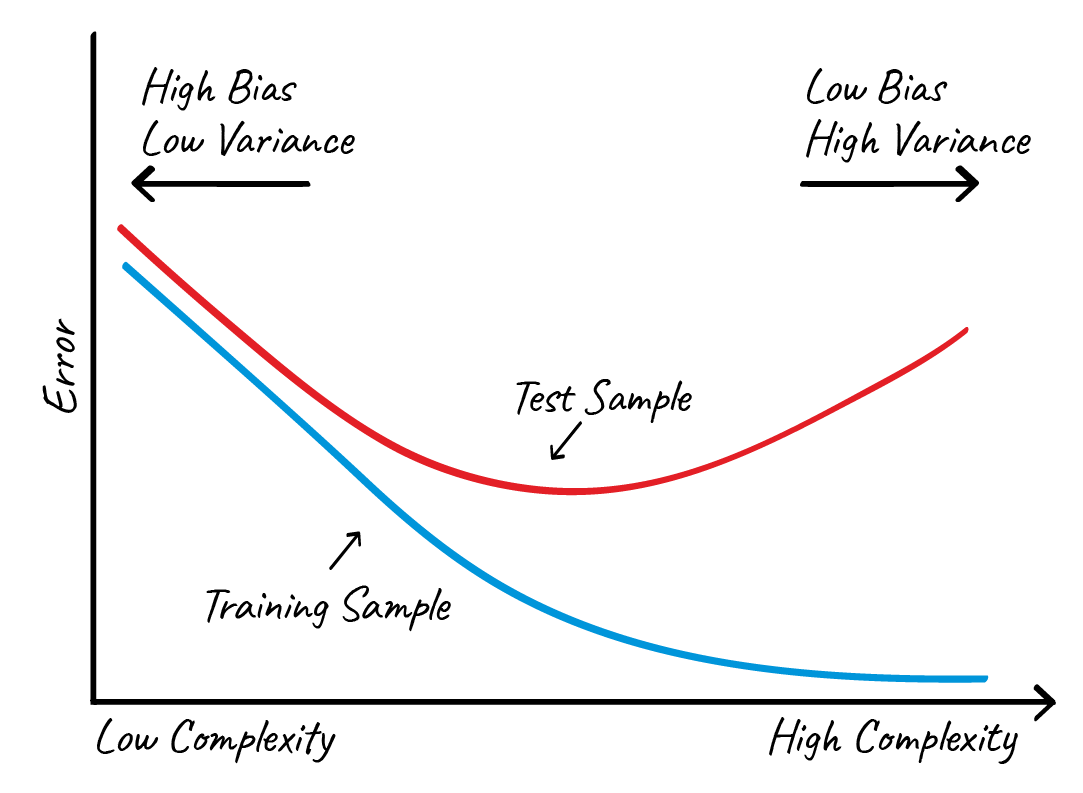
\includegraphics[width=4.5in]{chapters/ensemble.methods/figures/bias_variance.png}  
\caption{\textbf{The bias-variance tradeoff:} Train- vs. test errors as function of complexity of $h$}
\end{figure}

\subsection{Generalization Error Decomposition}
We have already encountered the generalization error decomposition when discussing linear regression problems (\todo{add link-reference to decomposition in regression}). There we have shown how we can decompose the MSE into the bias and variance components. Next, let us revisit the decomosition but for a general loss function. Let $h^{*}=argmin_{h\in\Hc} L_{\Dc}\left(h\right)$ and $h_S=\Ac\left(S\right)$ be the outout of a learning algorithm, then we can decompose the generalization error of the hypothesis returned by the learner as follows: 
\begin{equation}
L_{\Dc}\left(h_S\right) = \underset{\eps_{approximation}}{\underbrace{L_{\Dc}\left(h^{*}\right)}} + \underset{\eps_{estimation}} {\underbrace{L_{\Dc}\left(h_{S}\right)-L_{\Dc}\left(h^{*}\right)}}
\label{eqn:error_decomposition}
\end{equation}

\begin{itemize}
	\item The \textbf{approximation error} is $L_\Dc\left(h^*\right)$. Namely, the error of the hypothesis $h\in\Hc$ achieving the lowest generalization error. This term does not depend at all on our training sample and its size $m$. It depends only on the selection of $\Hc$. As we expand the hypothesis class to become richer we might find a better hypothesis for explaining the data. This error is what we already know as the \textbf{bias} error, induced by restricting the hypothesis class.
	\item The \textbf{estimation error} is $L_{\Dc}\left(h_{S}\right)-L_{\Dc}\left(h^{*}\right)$. Namely, it is the difference between the generalization error achieved by the selected hypothesis and the best hypothesis in $\Hc$. This term depends on the training set. \todo{Finish explaining why this is the variance term}
\end{itemize}        

\todo{Matan - Add explanation of how to properly create bias-variance curves}

\subsection{Lab: Bias-Variance Via Decision Trees}
\subsection{Lab: Bias-Variance Via Polynomial Fitting}
        
\section{Ensemble/Committee Methods}
\begin{quote}
	``A collective wisdom of many is likely more accurate than any one.'' —
	Aristotle, in {\em Politics}, circa 300BC
\end{quote}

Before diving into specific ensemble methods, let us analyze some mathematical properties of a committee based decision. This will give us insights into how committee based methods manage to inprove generalization. Consider a committee of $T$ members, which has to make a ``yes``/``no`` decision. Each member casts a vote, which with probability $p$ being correct and probability $1-p$ being wrong. Let's assume for simplicity that all members are ``equally wise'', so that $p$ is the same for all members. After all members vote, the committee's decision is simply the majority vote. For this setup we can ask questions such as:
\begin{itemize}
	\item What is the probability of the committee deciding the right decision?
	\item What would a typical decision be? and how consistent is it?
	\item How does the number of members in the committee influence the measures above?
	\item If committee members are not independent from one another, and influence each other's decisions, how does it influence the measures above?
\end{itemize}
~\\

\begin{exercise}
	Let $X_1,\ldots,X_T\overset{iid}{\sim}Ber\left(p\right)$ taking values of $\left\{\pm1\right\}$. What is the probability of the committee deciding right?
\end{exercise}
\begin{proof}
As the committee decides by a majority vote then the probability of the committee deciding right is the same as the probability of having more members deciding right than members deciding wrong: $$ \Prob\left(\text{Committee decides right}\right)=\Prob\left(\left|\text{Decided right}\right|>\left|\text{Decided wrong}\right|\right) $$
As each random variable takes a value in $\left\{\pm\right\}$ we could express the collective vote as $X=sign\left(\sum_{i=1}^TX_i\right)$. If the committee decided right, then ther are more members that voted right and $\sum_{i=1}^TX_i>0$ which means that $X=1$. On the otherhand, if the committee decided wrong, then more members voted wrong and $\sum_{i=1}^TX_i<=0$ which means that $X=-1$.

So, we conclude that: $$ \Prob\left(\text{Committee decides right}\right)=\Prob\left(X>0\right) $$
\end{proof}

\begin{exercise}
Let $X_1,\ldots,X_T\overset{iid}{\sim}Ber\left(p\right)$ taking values of $\left\{\pm1\right\}$ with $p>0.5$. Bound below the probability of the committee being correct.
\end{exercise}
\begin{proof}
W.l.o.g let us assume that the correct answer is $+1$ and denote $X=\sum_{i=1}^T X_i$. We are therefore interested in bounding from below $\Prob\left(X>0\right)$, which we will achieve by bounding below $\Prob\left(X\leq0\right)$. Notice that for any $a>0$ it holds that: $$ \Prob\left(X\leq 0\right)=\Prob\left(-aX\geq 0\right)=\Prob\left(e^{-aX}\leq e^0\right) $$

Now, using Markov's inequality $$ \Prob\left(X\leq 0\right) \leq \E\left[e^{-aX}\right]=\E\left[e^{-a\sum_i X_i}\right] \overset{iid}{=} \E\left[e^{-aX_1}\right]^T $$

Notice that as $X_1\sim Ber\left(p\right)$ over $\left\{\pm 1\right\}$it holds that: $$ \E\left[e^{-aX_1}\right] = pe^{-a} + \left(1-p\right)e^a \leq e^{a-p+pe^{-2a}}$$ where the last inequality is because $1+x\leq e^x$. Next, we use the inequality $x\ln\left(x\right)\geq \frac{x^2}{2}-\frac{1}{2}\quad x\in\left(x\right)$. For a selection of $a=\frac{1}{2}ln\left(2p\right)$ which is positive for $p>0.5$ we get that: 
$$
\begin{array}{ccl}
\Prob\left(X\leq0\right) & \leq & \E\left[e^{-aX_{1}}\right]^{T}\leq\exp\left(T\left(a-p+pe^{-2a}\right)\right)=e^{T\left(\frac{1}{2}ln\left(2p\right)-p+\frac{1}{2}\right)}=e^{Tp\left(-\frac{1}{2p}ln\left(\frac{1}{2p}\right)-1+\frac{1}{2p}\right)}\\
& \leq & e^{Tp\left(\frac{1}{2}-\frac{1}{2\left(2p\right)^{2}}-1+\frac{1}{2p}\right)}=e^{-\frac{Tp}{2}\left(\frac{1}{4p^{2}}-\frac{1}{p}+1\right)}=e^{-\frac{Tp}{2}\left(\frac{1}{2p}-1\right)^{2}}=e^{-\frac{T}{2p}\left(p-\frac{1}{2}\right)^{2}}
\end{array}
$$ Finally, we conclude that: $$\Prob\left(X>0\right) = 1-\Prob\left(X\leq 0\right) \geq 1-e^{\left(-\frac{T}{2p}\left(p-\frac{1}{2}\right)^2\right)}$$
\end{proof}


The above bound teaches us that for a committee of ``non-dump`` members (i.e. $p>1/2$) the probability of being wrong decays with a rate of $\Oc\left(\frac{1}{e^T}\right)$.Relating this to our learning scheme, it means that the confidence, $1-\delta$,  in our prediction increases dramatically as $T$ increases. Next, let us calculate what is a typical decision ($\E\left(X\right))$ and how consistent is it ($Var\left(X\right))$?

\begin{figure}[h!]
	\centering
	\animategraphics[loop,autoplay,width=0.8\textwidth]{1}{chapters/ensemble.methods/figures/bound_prob-}{0}{10}
	\caption{\textbf{Committee Decision - Correctness Probability:} Theoretical bounds and empirical results as function of $T,p$}
\end{figure}

\subsection{Uncorrelated Predictors}

\begin{exercise}
Let $X_1,\ldots,X_T\overset{iid}{\sim}Ber\left(p\right)$ taking values of $\left\{\pm1\right\}$ with $p>0.5$. What is the expectation and variance of $X=\frac{1}{T}\sum^T_{i=1}X_i$?
\end{exercise}
\begin{proof}
We begin with calculating the expectation and variance of each committee member:
$$
\begin{array}{rcl}
\E\left[X_{i}\right] & = & 1\cdot\Prob\left(X_{i}=1\right)+\left(-1\right)\cdot\Prob\left(X_{i}=-1\right)\\
& = & 2p-1\\
\\
Var\left(X_{i}\right) & = & \E\left[\left(X_{i}-\E\left[X_{i}\right]\right)^{2}\right]\\
& = & p\left(1-\left(2p-1\right)\right)^{2}+\left(1-p\right)\left(-1-\left(2p-1\right)\right)^{2}\\
& = & 4p\left(1-p\right)^{2}+4p^{2}\left(1-p\right)\\
& = & 4p\left(1-p\right)
\end{array}
$$

Then, for $X$:
$$
\begin{array}{rcl}
\E\left[X\right] & = & \frac{1}{T}\sum_{i}\E\left[X_{i}\right]=2p-1\\
Var\left(X\right) & = & \frac{1}{T^{2}}Var\left(\sum_{i}X_{i}\right)\overset{iid}{=}\frac{1}{T^{2}}\sum_{i}Var\left(X_{i}\right)=\frac{4}{T}p\left(1-p\right)
\end{array}
$$
\end{proof}

Therefore, when using a committee of independent members the expectation of decision remains the same while decreasing the variance at a rate of $\Oc\left(\frac{1}{T}\right)$. In other word, we are able to keep the same accuracy while increasing the confidence.

\todo{Add results of simulations }

\subsection{Correlated Predictors}
In practice, however, committee members rarely vote independently. So let us assume that each two members are correlated with equal correlation $\rho\in\left[0,1\right]$.

\begin{exercise}
Let $X_1,\ldots,X_T$ be a set of identically-distributed real-valued random variables such that: $Var\left(X_i\right)=\sigma^2$ and $corr\left(X_i,X_j\right)=\rho,\,\, i\neq j$. What is the variance of $X=\frac{1}{T}\sum_i X_i$?
\end{exercise}
\begin{proof}
As $X$ is the average of $T$ identically distributed random variables:
$$ Var\left(X\right)=Var\left(\frac{1}{T}\sum_i X_i\right)=\frac{1}{T^2}\left[\sum_i Var\left(X_i\right)+2\sum_{i<j}Cov\left(X_i,X_j\right)\right] $$
Recall that the correlation between two random variables is defined as: $$ corr\left(A,B\right)\coloneqq\frac{Cov\left(A,B\right)}{\sqrt{Var\left(A\right)Var\left(B\right)}} $$
and therefore for any $i\neq j$: $$ Cov\left(X_i,X_j\right)=corr\left(X_i,X_j\right)\sqrt{Var\left(X_i\right)Var\left(X_j\right)}=\rho\sigma^2 $$
Plugging this back into the variance:
$$ Var\left(X\right)= \frac{1}{T^2}\left[T\sigma^2+2{T \choose 2}\rho\sigma^2\right]=\frac{\sigma^2}{T}+\left(1-\frac{1}{T}\right)\rho\sigma^2=\rho\sigma^2+\frac{1}{T}\left(1-\rho\right)\sigma^2$$
\end{proof}

\todo{Add mathematical analysis of what does this mean}\\
\todo{Add simulation results - graph of variance as function of correlation + headmap of dependence on $T$}

All together, we have seen that given a committee of members that decides by majority vote, where decisions of members are correlated with correlation $\rho$ and each member is correct with probability $p$:
\begin{itemize}
	\item If $p>0.5$ the committee's decision improves with $T$ in two ways: higher probability of being right, and its decision will be more consistent.
	\item If $\rho>0$ then increasing $T$ will increase the probability of the committee's decision being right up to a certain point,
\end{itemize}

\subsection{Committee Methods In Machine Learning}
Going back to machine learning, suppose we have $T$ training samples $S_1,\ldots,S_T$ of size $m$ chosen independently from $\Xc$ according to some distribution $\Dc$. Let $\Ac$ be a learning algorithm and train it on each of the training samples, to obtain $h_{S_1},\ldots,h_{S_T}$. Let us consider $h_{S_t}\left(x\right)$ for some $x\in\Xc$. As $S_t\iid\Dc^m$ we can think of the training set as a random variable. This means that the also $h_{S_t}$ obtained by training $\Ac$ over $S_t$ is a random variable. Lastly, it means that we can think of the prediction $h_{S_t}\left(x\right)$ as a random variable, which has some distribution. In addition, notice that as the training samples are chosen independently, predictions of different $h_{S_t}$ over $x$ are also independent random variables. So, if we use $h_{S_1},\ldots,h_{S_T}$ in a committee we have the situation described above. The generalization loss will improve with $T$, tending to $0$ as $T\rightarrow\infty$. In addition, the variance of the prediction will decrease as $1/T$.
\\~\\
However, in batch learning we don't have $T$ training samples, but rather just one, so how would we accuire such different hypotheses? We cannot train $\Ac$ over $S$ multiple times as we will get identical predictions, which are perfectly correlated. Instead, what we would like to do is to create $T$ training samples from the original one. If we could mimic fresh independent draws of new traning samples of size $m$ according to $\Dc$.

\begin{definition}[Committee Methods]
Let $\Ac$ be some learner predicting labels in $\left\{\pm\right\}$. A committee method over $\Ac$ is the function: $$ h\left(x\right)=sign\left(\sum^{T}_{t=1}h_t\left(x\right)\right) $$
\end{definition}
That is, in committee methods (or ensembles) we take an existing ``base`` learner and apply it ot a sequence of $T$ training samples. For the remaining of this chapter we will introduce two very different ideas for building the committee member rules.


\section{Bagging}
\subsection{Bootstrapping} \label{bootstrap}
For the first committee method we begin with introducing a concept from statistics: \textbf{Bootstrapping}. It is any test or metric that by repeated random sampling \textbf{with replacement} of a sample is able to more accurately infer parameters of the sample distribution.
~\\
\todo{general bootstrap example for some parameter estimation}

~\\
So, given a training sample $\trainset$ we are going to construct a new training sample, called a \textit{bootstrap sample} $S^{*1}$. We sample $m$ times from $S$ \textbf{with replacement} and denote this ``new`` sample by: $$ S^{*1}=\left\{\left(\x_i^{*1},y_i^{*1}\right)\right\}^m_{i=1} $$
Of course, since we sampled from $S$ with replacements, there might be repeated samples in $S^{*1}$, even if $S$ itself had no repeated samples. Now we can repeat this process $B$ times, obtaining $B$ training samples, each of length $m$: $S^{*1},\ldots,S^{*B}$. The samples in the $b$-th training sample will be denoted $$ S^{*b}=\left\{\left(\x_i^{*b},y_i^{*b}\right)\right\}^m_{i=1} $$

Using the newly created bootstrap samples we can now train our base learner $\Ac$ over each one separatly, obtain $B$ prediction rules and form an ensemble. But so how is it that bootstrap actually works? Assume for a moment that samples in our learning problem are i.i.d samples from an unknown distribution $\Dc$ over $\Xc\times\Yc$. We are hoping that each Bootstrap from $S$ somehow behaves like a fresh iid sample from $\Dc$ itself. Given a training sample $S$ (assume for simplicity that all the points of $S$ are distinct) let's define the \textbf{empirical distribution} $\widehat{\Dc}_S$ induced by $S$ on $\Xc\times\Yc$ as the following probability distribution
on $\Xc\times\Yc$: for a subset $C\subset\Xc\times\Yc$, define:
$$
\widehat{\Dc}_S( (X,Y)=(x,y) ) \coloneqq 
\begin{cases}
\frac{1}{m} & (x,y)\in S\\ 
0 & (x,y) \notin S
\end{cases}
$$
or equivalently, for any $C\subset\Xc\times\Yc$:
$$
\widehat{\Dc}_S(C)\coloneqq \frac{| C \cap S |}{m}	
$$
Observe that this is equivalent to putting a probability mass of $1/m$ on each of the points of $S$, and zero mass on all other points in $\Xc\times\Yc$. \textbf{Now observe that a bootstrap sample $S^{*b}$ is just an iif draw of $m$ points} from the empirical distribution $\widehat{\Dc}_S$ induced by the one training sample we have, $S$. As $m$ grows, namely as $S$ becomes larger, the empirical distribution $\widehat{\Dc}_S$ converges in distribution to $\Dc$. The idea behind the bootstrap is that, if $\widehat{\Dc}_S$ is not so different from $\Dc$, then $m$ iid draws from $\widehat{\Dc}_S$ is a good approximation to $m$ iid draws from $\Dc$. One way to see the convergence of the empirical distribution to the underlying distribution is on the real line:

\todo{Have code for simulation!}
\begin{exercise}
In simulation, take $\mathcal{F}$ to be, $\Nc(0,1)$. For each value $m=10,100,1000$, draw a sample and plot its empirical CDF - and overlay the CDF of $\Nc(0,1)$. Recall that on the real line, convergence in distribution is equivalent to convergence of the CDFs to a limiting CDF at the continuity points of the limiting CDF.
\end{exercise}

\begin{figure}[h!]
	\centering
	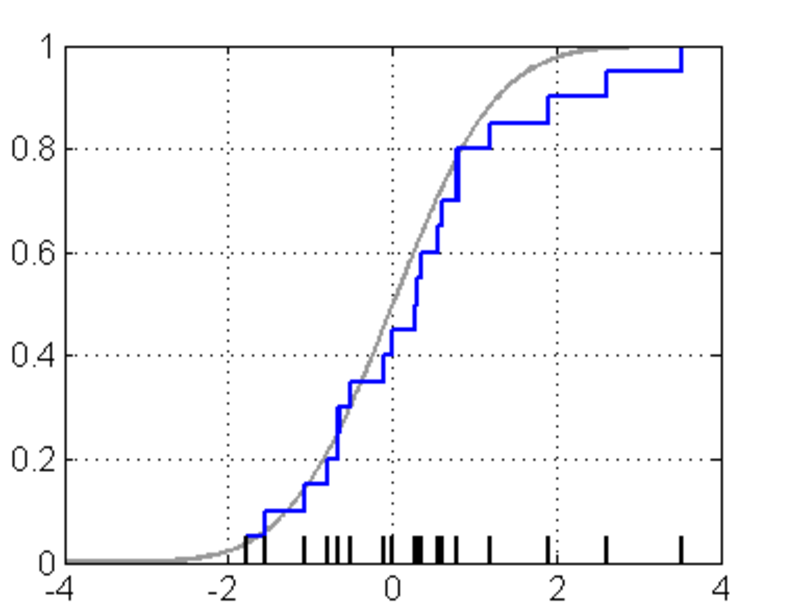
\includegraphics[width=3.5in]{chapters/ensemble.methods/figures/ecdf.png}  
	\caption{CDF of a probability distribution on the real line, and empirical CDF of an i.i.d sample from that distribution. Black lines on the horizontal axis show the random sample.}
	\label{ecdf}
\end{figure}
\subsection{Bootstrapping for Bagging}
The idea of Bootstrap samples can be used whenever we would like to create new artificial samples from our only training sample $S$. It has many uses throughout machine learning, statistics and data science. \textbf{Bagging} is a nickname for a straightforward use of the Boostrap in machine learning, to improve accuracy of an existing supervised machine learning algorithm.

~\\
We start with a ``base`` learning algorithm $\Ac$ and a training sample $S$. We choose $T$ (later discussed how) and form $T$ bootstrap training samples, $S^{*1},\ldots, S^{*T}$, each of size $m$. We then train our learner \textbf{separately} on each of the $T$ bootstrap training samples. We form the committee $h_{S^{*1}},\ldots,h_{S^{*T}}$ and store all $T$ trained models. When we need to classify a new test sample $x\in\Xc$, we run $x$ through all the rules and classify using the majority vote of the committee,
$$
h_{bag}(x) \coloneqq sign\left( \sum_{t=1}^T h_{S^{*t}} (x)\right)
$$

For example, if we run Bagging on top of the Decision Tree classifier, we'll obtain a committee of decision trees: \todo{Add graph+code for num. Bootstraps vs Test error}
\begin{figure}[h!] %TODO - width to percentages
	\centering
	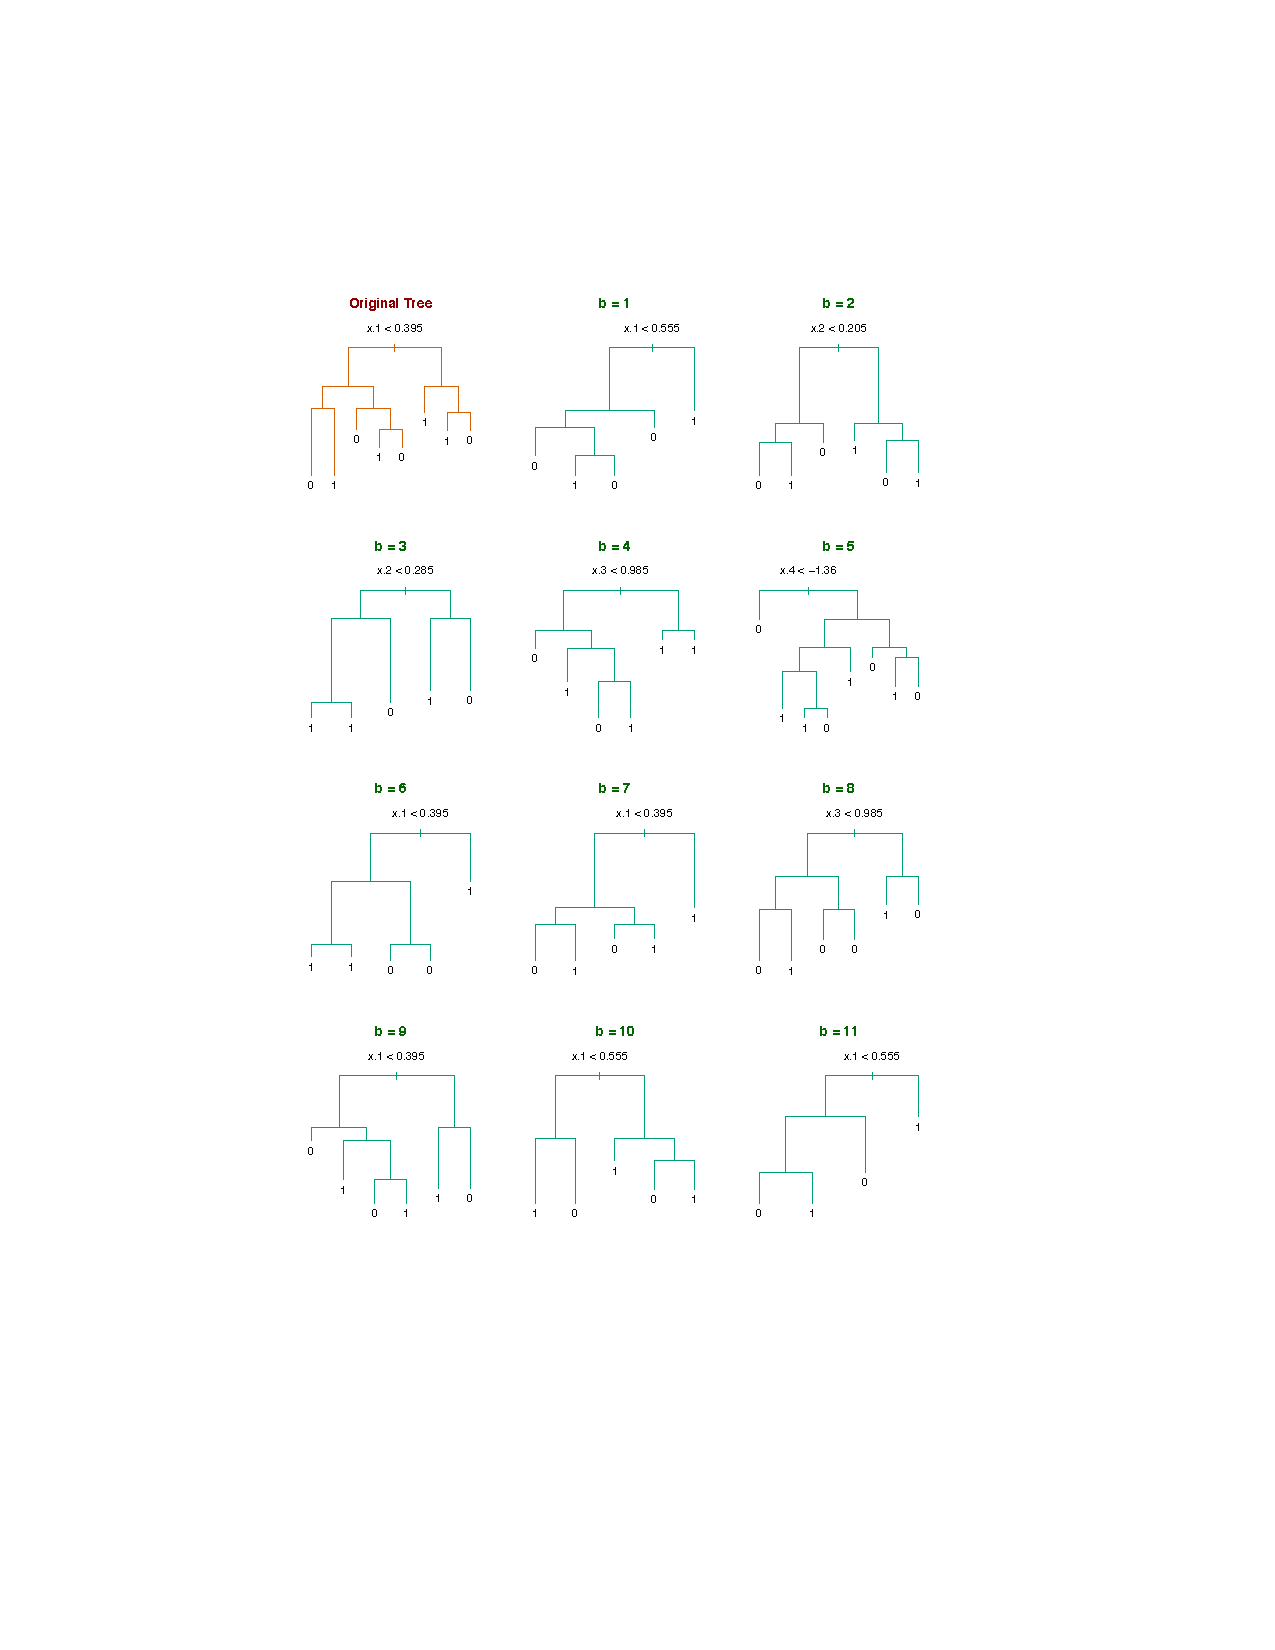
\includegraphics[width=1.8in]{chapters/ensemble.methods/figures/many_trees.png}
		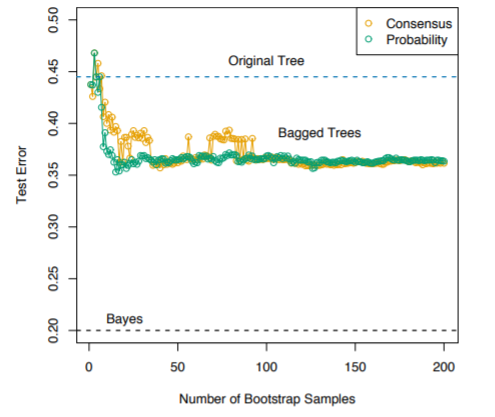
\includegraphics[width=3.5in]{chapters/ensemble.methods/figures/bagging.png}
	\caption{Collection of Bagged Decision Trees. (Source: ESL)}
	\label{bagging_sim}
\end{figure}

~\\
Note that our learner $\Ac$ must know how to handle repeated samples. We may have them anyway in $S$, but running on a bootstrap sample we are sure to have them. Some
learning algorithms suffer when there are repeated samples - as they cause numerical problems (for example, linear and logistic regression), while for others it isn't a problem (for example, decision trees and $k$-NN).

\subsection{Bagging Reduces Variance}
We saw that a committee majority vote reduces variance, but as seen in Figure \ref{ecdf} only to a certain degree. The amount of variance reduced is determined by the correlation between committee members. So, we can expect bagging to reduce variance as $T$ increases (and therefore to reduce the generalization error) but only proportionate to the correlation between the bagged prediction rules.

\subsection{Random Forests Bagging and De-correlating Decision Trees}
So, bagging can be improved by somehow de-correlating the bagged prediction rules. How do we de-correlate the committee members - namely, cause their predictions somehow to be less correlated? One way to do this is by handicapping (restricting) each learner a little, in a random way, and hope that the performance gain (in bagging them) due to de-correlation is more than the performance loss to each learner by handicapping. The most well know example of this principle is \textbf{Random Forests}

~\\
Recall the Decision Tree classification algorithm over $\Xc=\R^d$. We have a training sample $S$ with $m$ points. The Random Forest classifier is obtained by using Bagging on top of the Decision Tree algorithm, \textbf{with an important twist} for de-correlation: the algorithm has a tuning parameter $k\leq d$. When growing each decision tree, in each split, we choose $k$ out of the $d$ coordinate uniformly at random, and only choose the split among these $k$ coordinates. Formally:

\todo{add styled pseudo code for random forests}

This de-correlation trick works: pretty much on every classification problem you'll work on, you'll observe something like the next plot: Bagging trees is
much better than a single tree, and Random Forest (Bagging with the de-correlation trick) is better than just Bagging trees.

\todo{Own code for graph without gradient boosting + update caption}
\begin{figure}[h!]
	\centering
	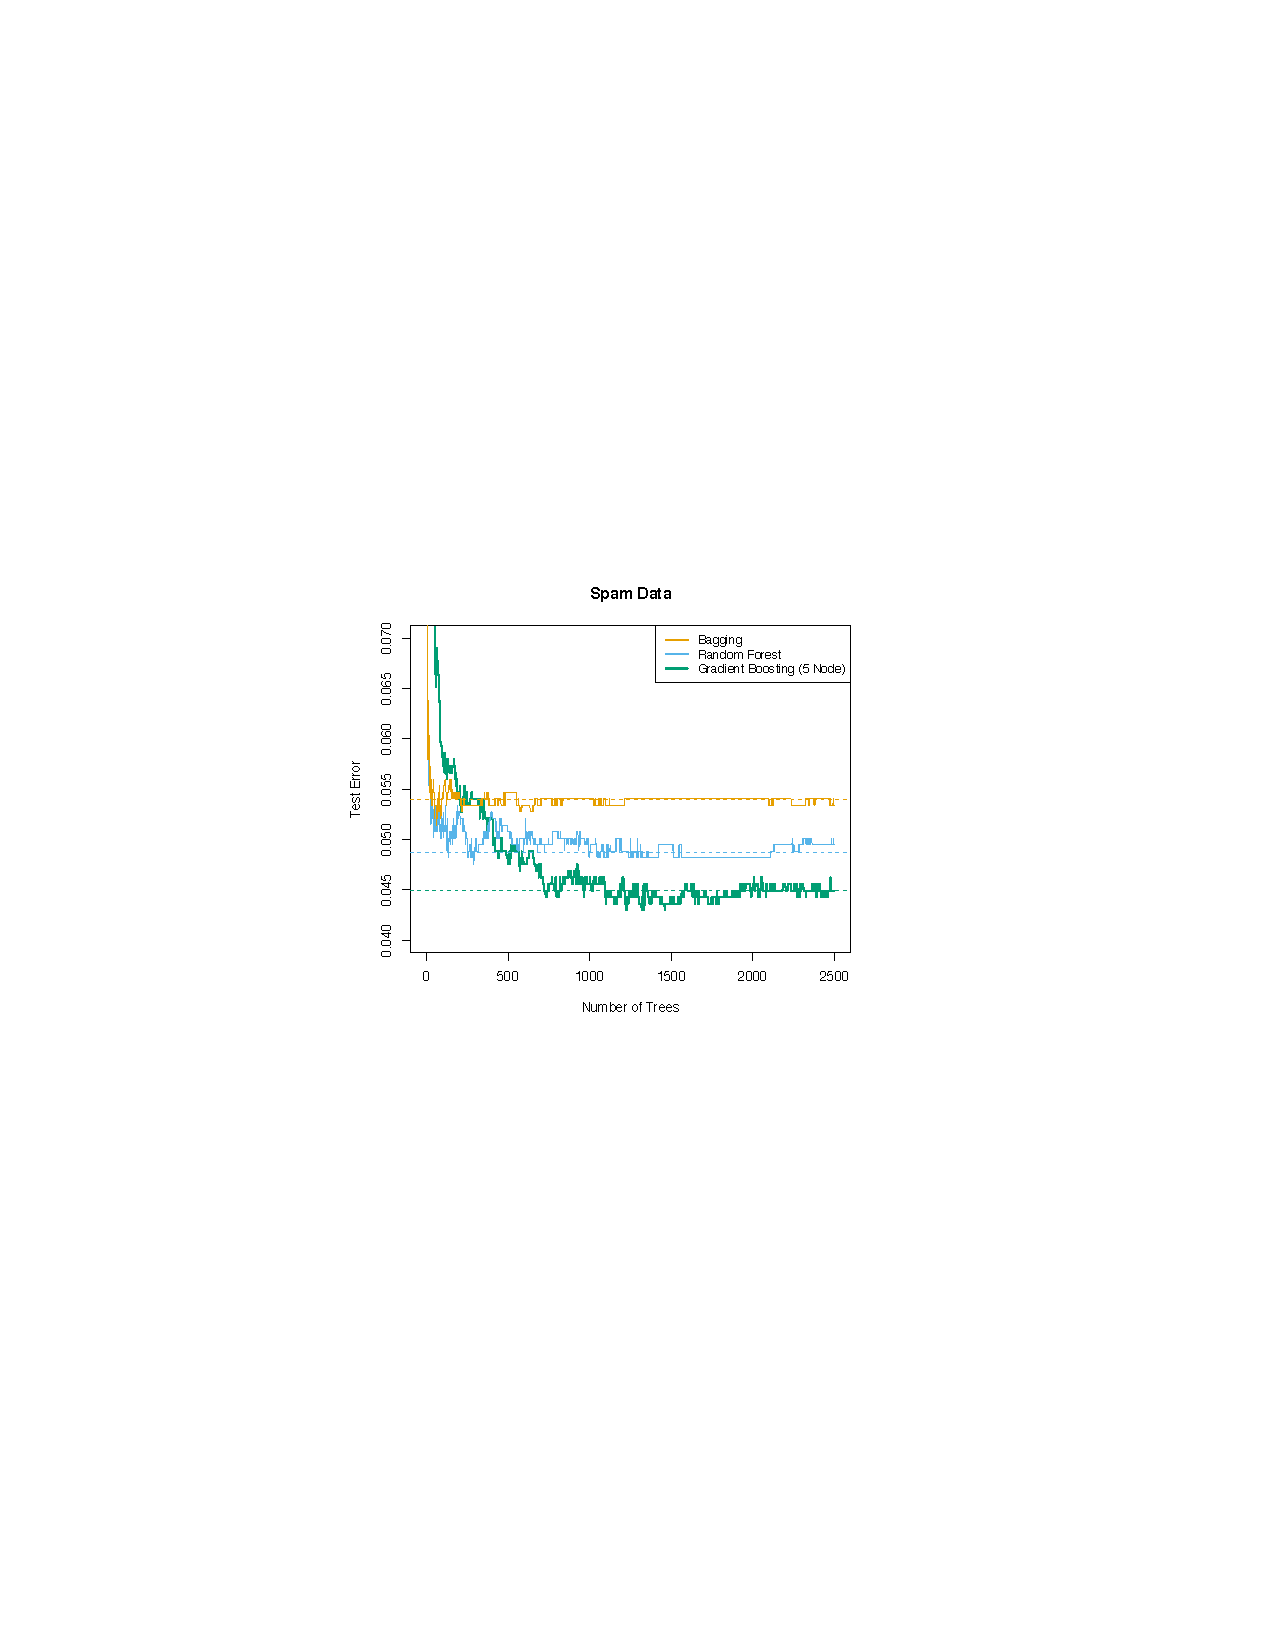
\includegraphics[width=4in]{chapters/ensemble.methods/figures/bagging_vs_rf.png}
	\caption{Test error of simple Bagging of decision trees (no de-correlation), Random Forests, and Gradient Boosting of Trees. (Source: ESL)}
\end{figure}

\subsubsection{Bagging - Discussion Points}
\begin{itemize}
	\item \textbf{Can Bagging harm our prediction?} Always remember that a committee of fools (a committee where each member has probability $p<0.5$ to make the right decision) makes worse decisions than a single member. So, when our base learner is so poor that its generalization loss is less than $0.5$ we shouldn't use Bagging.
	\item \textbf{What are the disadvantages of Bagging?} As we train not one but $T$ models we need to train all $T$ of them. This directly increases time complexity by a factor proportionate to $T$. In addition, for predictions, as we need all $T$ models we must store all $T$ of them. Lastly, we loose interpretability as it is much harder to understand why the committee made the decision. We need to understand the decision of each of the $T$ members.
	\item \textbf{Parallelizem} From the computational perspective, it is important to note that Bagging in general (and Random Forests in particular) is \textbf{embarrassingly parallelizable}. When training a Bagging model with $T$ committee members, we can use $T$ machines in parallel, each using its own random seed to select Bootstrap samples (and random splits, in Random Forest). The machines do not need to interact; when each machine is done, it returns the committee member $h_t$ to the master node.
	\item \textbf{Predicted Class Probabilities:} Can we use the \textbf{proportion} of the committee members who voted $+1$ as a predicted class probability? Estimated class probabilities are estimates of $\Prob\left\{ Y=+1,|\, X=x \right\}$. The proportion of members who voted $+1$ estimates $\Prob\left\{ h_S(x)=+1 \right\}$, which is a different quantity.
\end{itemize}

\section{Boosting}
Bootstrap was magic of the following kind: we take a single training sample $S$ and turn it into many training samples. Bagging uses this magic by training a model over these ``new`` training samples, and averaging the result to reduce the variance and hence the generalization error. Boosting is magic of a different kind. In Boosting we take a ``weak`` learning algorithm, an algorithm with better-than-random but possibly not so good accuracy (i.e. generalization error) and \textbf{boost} it using a clever committee method to obtain a learning algorithm with good accuracy. 
\\~\\
The core idea of Boosting is a completely different idea for creating a committee of prediction rule from a base learning algorithm $\Ac$ and a single training sample $S$. In Bagging, we ``pretended`` to have fresh training samples $S_1,\ldots,S_T$, and each committee member trained on a different sample. In Boosting, we go even further and ``pretend`` to have \textbf{different underlying distributions} $\Dc$ from which the training sample is drawn. More specifically, in Boosting each committee member $h_t$ is the result of running $\Ac$ against a training sample $S_t$ that mimics an i.i.d sample of size $m$ from a \textbf{different distribution} $\Dc^t$. Whereas in Bagging each committee member is trained independently of all other members, in Boosting the committee members are trained sequentially, one after the other, and each is an improvement, in some sense, on the previous one. 

The clever idea behind Boosting is that after we finish training $h_t$, based on the distribution $\Dc^t$, we update the distribution in a way that \textbf{increases the distribution at training samples where $h_t$ was wrong}. This way, $h_{t+1}$ will try very hard not to be wrong on those particular samples, and so on. 

\todo{ Add Animation of Boosting iterations progress}

But first, we have to understand  what is meant by ``running $\Ac$ against the training sample $S$ with distribution $\Dc^t$``. One way to interpret this is to take a \textbf{weighted Bootstrap} sample from $S$, where the probability of selecting $(x,y)\in S$ is proportional to $\Dc^t(x,y)$. A simpler way to interpret this is as follows. If $\Ac$ uses the ERM principle, say for standard misclassification ($0-1$ loss), namely, looking to minimize the empirical risk,
$$ L_S(h) = \sum_{i=1}^m \indc{y_i \neq h(\x_i)} $$
then we can use $S$ itself (and not any bootstrap sample) and have the base learner minimize the \textbf{weighted} empirical risk
$$ L_{S,\Dc^t}(h) = \sum_{i=1}^m \Dc^t_i\indc{y_i \neq h(\x_i)} $$
where for each $(\x_i,y_i)\in S$ we write $\Dc^t_i \coloneqq \Dc^t(\x_i,y_i)$, so that $\sum_{i=1}^m \Dc^t_i =1$.
\\~\\
Observe that these two interpretations are equivalent in expectation. Indeed, the expected number of times for a sample $(\x_i,y_i)$ to appear in the weighted Bootstrap sample is $\Dc^t_i$, and so it would (in expectation) appear $\Dc^t_i$ times in the empirical risk sum. 
\\~\\
Note that we usually prefer second option (using weighted empirical risk) to the first option (using weighted bootstrap). It's more computationally efficient, and does not require worrying about repeated samples. However, the first option (using weighted bootstrap) is always available. The second option (using weighted empirical risk) is not always possible, and is implemented ad-hoc for the particular base learner we are boosting.

\todo{add solution? + fix bullets}
\begin{exercise}
To help you understand this point, describe how you would implement a Decision
Tree with each of the two methods:
\begin{itemize}
	\item Using weighted empirical risk: How would you change the Decision Tree
	algorithm we've seen (CART) to work with a given weight vector $\Dc^t$ over
	the training sample $S$? (Hint: what is the best splitting now that we have
	weights?)
	\item Using weighted Bootstrap: How would you How would you change the Decision Tree
	algorithm we've seen (CART)  to work with a given weight vector without
	changing the splitting algorithm, namely, by giving the algorithm a
	different training sample selected by weighted Bootstrap? Will the algorithm
	work with repeated samples?
\end{itemize}
\end{exercise}

\subsection{AdaBoost Algorithm}
The original Boosting meta-algorithm is known as \textbf{Ada}ptive \text{Boost}ing:
\todo{Write pseudo down instead of image}
\begin{figure}[h!]
	\centering
	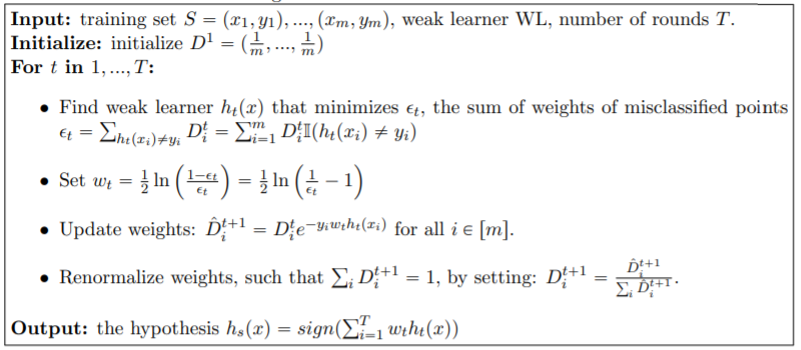
\includegraphics[width=6in]{chapters/ensemble.methods/figures/adaboost_pseudo.png}
\end{figure}

The idea is simple: from iteration $t$ to iteration $t+1$, we want to \textbf{increase} the weights of samples misclassified  by $h_t$ (where $y_i h_t(\x_i)=-1$) and \textbf{decrease} the weights of samples correctly classified by $h_t$. We want to make the classification problem ``maximally hard`` in the sense that weighted empirical
risk of $h_t$, with respect to the updated weights $\Dc^{t+1}$, is the worse possible, namely $1/2$. Finally, the prediction rules vote in the committee with weights $w_t$.

\begin{claim}
For the weighting factor of $w_t=\frac{1}{2}ln\left(\eps_t^{-1}-1\right)$ and $\varepsilon=\sum_{i=1}^m\Dc^t_i\cdot\indc{y_i\neq h_t\left(\x_i\right)}$ the weighted empirical risk of $h_t$ with respect to $\Dc^{t+1}$ is $1/2$: $$\sum_{i=1}^m\Dc_i^{t+1}\cdot\indc{y_i\neq h_t\left(\x_i\right)}=\frac{1}{2} $$
\end{claim}
\begin{proof}
	Directly expressing the weighted empirical risk:
$$
\begin{array}{ccl}
\sum_{i=1}^{m}\Dc_{i}^{t+1}\cdot\indc{y_{i}\neq h_{i}\left(\x_{i}\right)} & = & \frac{\sum_{i=1}^{m}\Dc_{i}^{t}\exp\left(-\w_{t}y_{i}h_{t}\left(\x_{i}\right)\indc{y_{i}\neq h_{t}\left(\x_{i}\right)}\right)}{\sum_{j=1}^{m}\Dc_{j}^{t}\exp\left(-\w_{t}y_{j}h_{t}\left(\x_{j}\right)\right)}\\
\\
& = & \frac{\exp\left(\w_{t}\eps_{t}\right)}{\exp\left(\w_{t}\eps_{t}\right)+\exp\left(-\w_{t}\right)\left(1-\eps_{t}\right)}\\
\\
& = & \frac{\eps_{t}}{\eps_{t}+\exp\left(-2\w_{t}\right)\left(1-\eps_{t}\right)}\\
\\
& = & \frac{\eps_{t}}{\eps_{t}+\frac{\eps_{t}}{1-\eps_{t}}\left(1-\eps_{t}\right)}=\frac{1}{2}
\end{array}
$$
\end{proof}

\subsection{PAC View of Boosting - Weak Learnability}
Historically, Boosting appeared as an answer to a fascinating question for which we first need to define \textbf{Weak Learnability}:\\

\begin{definition}[$\gamma$-weak-learner] 
A learning algorithm $\Ac$ is a $\gamma$-weak-learner for an hypothesis class $\Hc$ if there exists a function $m_\Hc:(0,1)\to\N$ such that for every $\delta\in\left(0,1\right)$, for every distribution $\Dc$ over the sample space $\Xc$, and for every labeling function $f:\Xc\to\left\{ \pm \right\}$, if the realizabiity assumption holds with respect to $\Hc,\Dc,f$, then when running $\Ac$ on a training sample of $m\geq m_\Hc(0,1)$ i.i.d samples drawn according to $\Dc$ and labeled by $f$, the algorithm returns an hypothesis $h_S=\Ac(S)$ such that with probability at least $1-\delta$ (with respect to choice of the training sample $S$), we have $L_{\Dc,f}(h_S) \leq 1/2-\gamma$. 
\end{definition}

\begin{definition}
An hypothesis class $\Hc$ is $\gamma$-weak-learnable if there exits a $\gamma$-weak-learner for $\Hc$.
\end{definition}

How is this different than PAC-learnability? If an hypothesis class $\Hc$  is PAC-learnable, then for \textbf{every} $(\eps,\delta)$ there exists a learner $\Ac$. This means that we can learn and generalize a labeling function from $\Hc$ to any accuracy $\eps$ we want. But if $\Hc$ is $\gamma$-weak-learnable, for any $\delta$ \textbf{and just for $\eps=1/2-\gamma$} there is a learner $\Ac$. We may not be able to find a learner that has better accuracy (lower $\eps$). 
\\~\\
The question that motivated Boosting was the following: 
\begin{itemize}
	\item Suppose that $\Hc$ is PAC-learnable. Then we know that the rule $ERM_{\Hc}$ will learn (namely, will be probably approximately correct etc) with a near-minimal number of samples.
	\item But what if $ERM_\Hc$ is computationally hard? (we've seen examples)
	\item Assume we can find a \textbf{simple} hypothesis class (a ``base hypothesis class``) $\Hc_{base}$, such that $ERM_{\Hc_{base}}$ (choosing the hypothesis in $\Hc_{base}$ with lowest empirical risk) is computationally efficient, and is $\gamma$-weak-learner for $\Hc$ for some $\gamma$.
	\item This means that we have a computationally efficient way to learn with accuracy $1/2-\gamma$, for some $\gamma$. Maybe we can't find an efficient learner with better $\gamma$.
	\item Is there a way to \textbf{boost} $ERM_{\Hc_{base}}$ in a computationally efficient way, and create a computationally efficient learner $\Ac$ which is close to minimizing $ERM$ over $\Hc$?
\end{itemize}~\\
For example, think about Decision trees. We saw that the ERM learner is not computationally feasible on this hypothesis class. But a small tree may be able to achieve accuracy (over a sample labeled by a larger tree) which is not great, but better than random. Well, as the following theorem shows, Adaboost does just that (for the full proof refer to UML 10.2)
\begin{theorem}
Let $S$ be a training set. Assume that at each iteration of Adaboost, the base learner returns a prediction rule (hypothesis $h_t$) for which the weighted empirical risk satisfies:
$$ \sum_{i=1}^m \Dc^{t}_i\indc{y_i \neq h(\x_i)} \leq \frac{1}{2}-\gamma $$
Then the (standard, non-weighted) empirical risk of the output prediction rule of Adaboost, $h_{boost}$, (the weighted committee vote) satisfies:
$$ L_S(h_{boost}) \equiv \frac{1}{m}\sum_{i=1}^m \indc{y_i \neq h_{boost}(\x_i)} \leq e^{-2\gamma^2 T }$$
\end{theorem}

\subsection{Bias-Variance in Boosting}
The hope is, of course, that we're not overfitting, so that low empirical risk will imply low generalization loss. Suppose we run $T$ iterations of Adaboost over a learner $\Ac_{base}$ that returns hypothesis from $\Hc_{base}$. What is the effective hypothesis class we have now, and how large is it? Well, Adaboost with $T$ iterations will return a function from the hypothesis class  
$$\Hc_T = \left\{ \x\mapsto \sum_{t=1}^Tw_t h_t(\x) \,| \, w_1\ldots w_T\in[0,\infty),\,\, \sum_t w_t=1,\,\, h_1\ldots,h_T\in\Hc_{base}\right\}$$
namely convex combinations of hypotheses from $\Hc_{base}$. So $\Hc_t$ becomes larger (contains more functions) as $T$ grows. But it doesn't grow too fast with $T$. 
\\~\\
For example, we have a canonical way to measure the ``size`` of $\Hc_T$. While we won't go into the details, under certain conditions, $VCdim(\Hc_T)$ is roughly $T\cdot VCdim(\Hc_{base})$. So we can expect Boosting to increase the variance (compared with the base learner) as $T$ increases, but ``not too fast``. 
\\~\\
On the other hand, it's clear that Boosting decreases bias - that is obvious from the fact that the empirical risk decreases as $T$ grows - indeed $\Hc_T$ is able to come closer and closer to the labeling function on the training set. And the fact that empirical risk decreases \textbf{exponentially} with $T$ tells us that bias decreases quite quickly. Overall, Boosting typically decreases bias much faster than it increases variance, which is why it typically improves generalization loss quite dramatically. But a question remains: If we use $T$ too large, will boosting overfit? 
